%\usepackage[T1]{fontenc}
%\usepackage[utf8]{inputenc}

%!TEX ROOT=../diploma-thesis.tex

\chapter{Návrh}\label{ch:navrh}

V této kapitole ...

\section{Formalizace architektury orientované na služby}

\subsection{Join-points}

\begin{figure}
    \centering
    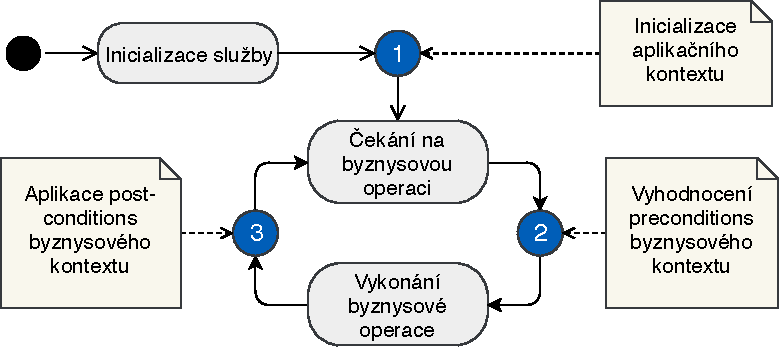
\includegraphics[keepaspectratio=true, width=0.8\linewidth]{figures/join-points.pdf}
    \caption{Diagram životního cyklu služby a identifikovaných join-pointů}
    \label{fig:join-points}
\end{figure} % TODO: popsat

\subsection{Advices}

\subsection{Pointcuts}

\subsection{Weaving}

\section{Architektura frameworku}

\section{Zachycení byznysového konextu}

Přístup ADDA doporučuje popsat byznysová pravidla pomocí
vlastního, na míru šitého, doménově specifického jazyka~\cite{cemus2015automated}.
V našem případě můžeme jazykem DSL popsat kompletně i celý
byznysový kontext.

\section{Metamodel byznys kontextu}\label{sec:metamodel}

\begin{figure}
    \centering
    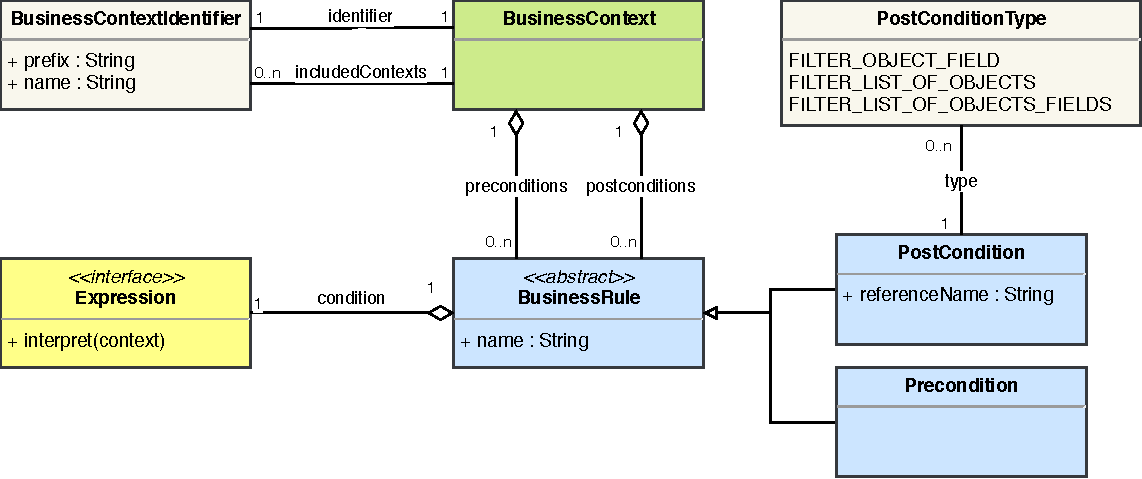
\includegraphics[keepaspectratio=true, width=\linewidth]{figures/business-context-metamodel.pdf}
    \caption{Diagram tříd metamodelu byznysového kontextu}
    \label{fig:business-context-metamodel}
\end{figure} % TODO: popsat

\section{Expression}

\section{Registr byznys kontextů}

\begin{figure}
    \centering
    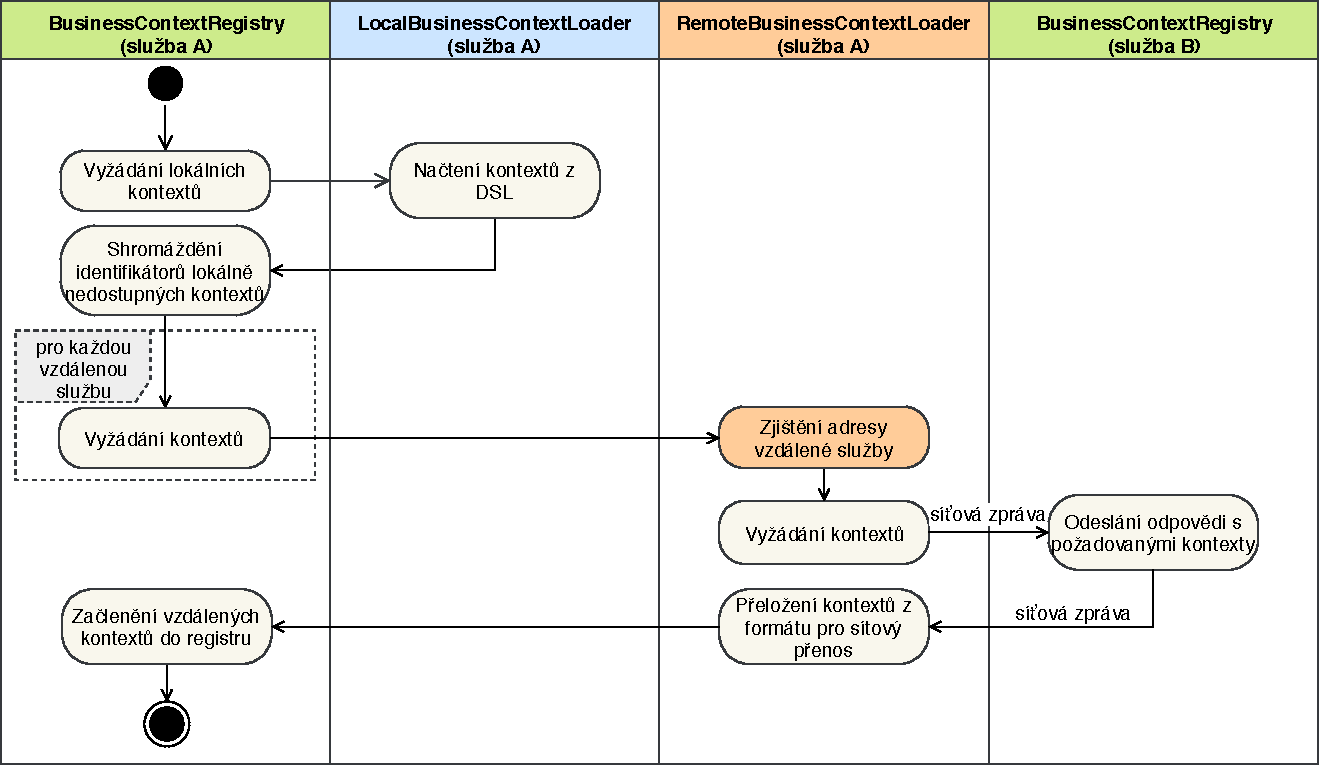
\includegraphics[keepaspectratio=true, width=0.8\linewidth]{figures/business-context-loading.pdf}
    \caption{Diagram procesu inicializace byznysových kontextů}
    \label{fig:business-context-loading}
\end{figure} % TODO: popsat

\section{Byznys kontext weaver}

\begin{figure}
    \centering
    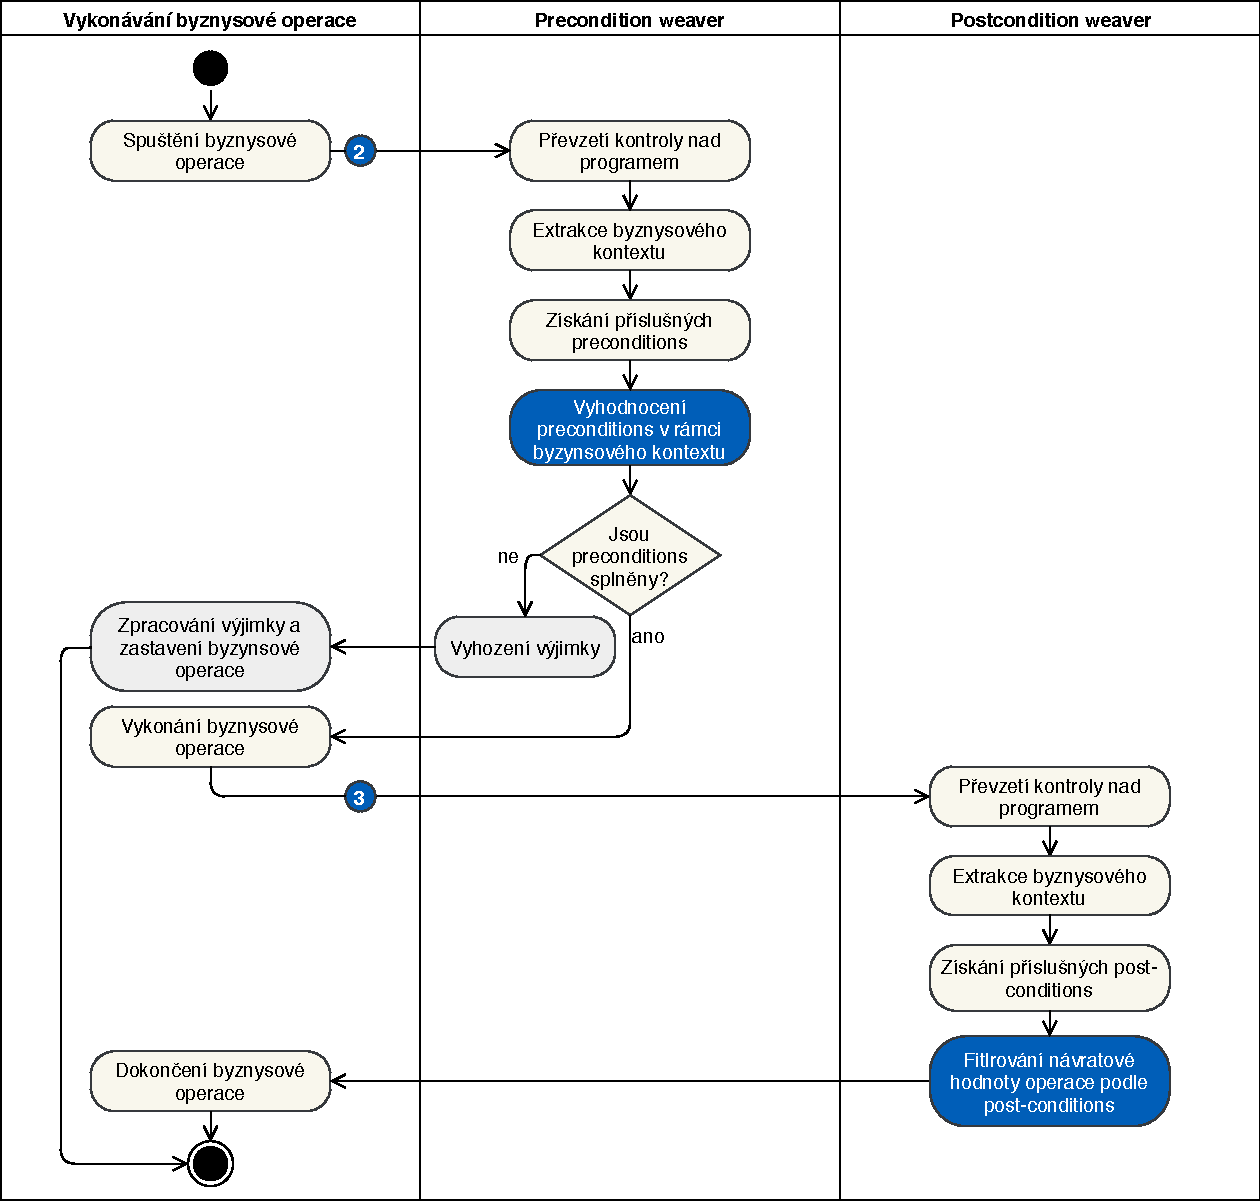
\includegraphics[keepaspectratio=true, width=0.8\linewidth]{figures/business-rules-weaver.pdf}
    \caption{Diagram aktivit weaverů byznysových pravidel}
    \label{fig:business-rules-weaver}
\end{figure} % TODO: popsat

\section{Centrální správa byznys kontextů}

\begin{figure}
    \centering
    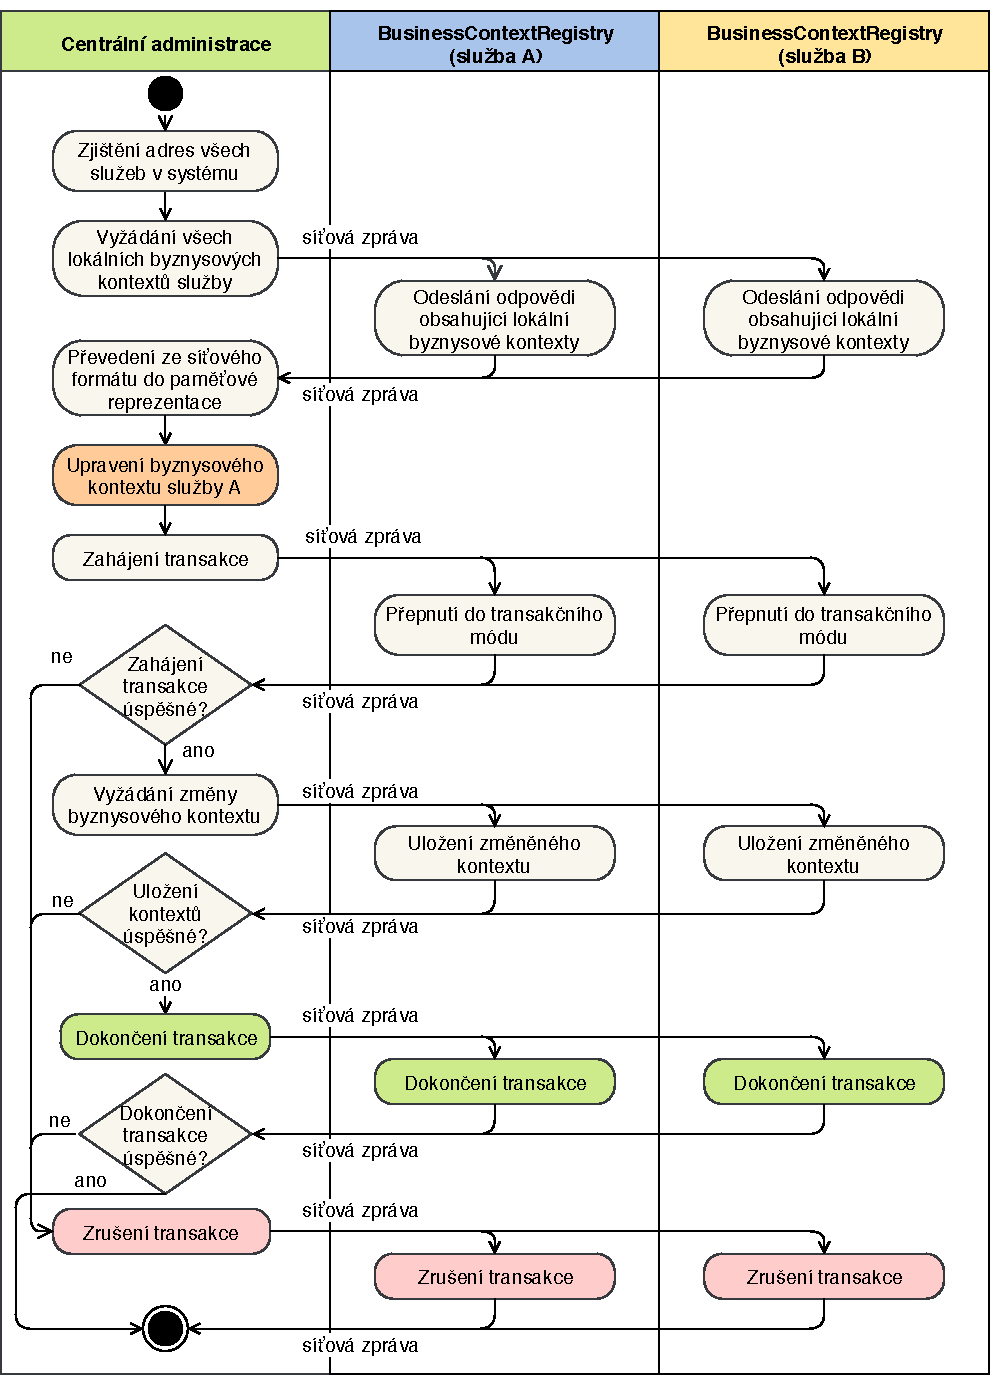
\includegraphics[keepaspectratio=true, width=0.8\linewidth]{figures/business-context-management.pdf}
    \caption{Diagram procesu centrální správy byznysových kontextů}
    \label{fig:business-context-management}
\end{figure} % TODO: popsat

\subsection{Uložení rozšířeného pravidla}

\goal{Diskutovat chaining vs. direct update}
% TODO: napiš mě

\section{Service discovery}

\goal{Popsat nezávislost na service discovery}
